% pointer jumping on a forest of two trees
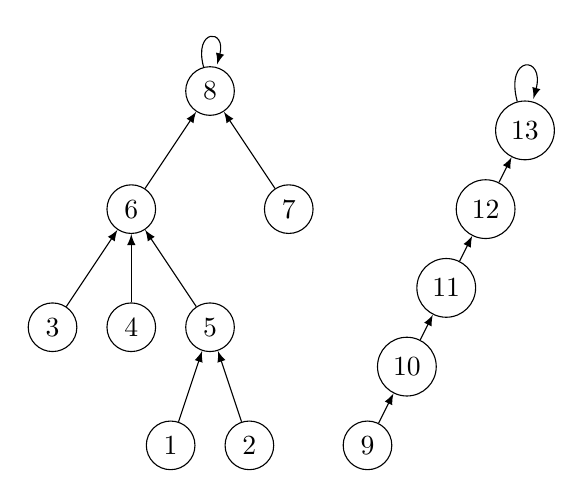
\begin{tikzpicture}
    [
        ->,>=latex,
        vertex/.style={circle, draw, scale=1, minimum size=3ex,},
        edge/.style={-latex,},
    ]

    % t1
    \node (1) at (1.5,0) [vertex] {$1$};
    \node (2) at (2.5,0) [vertex] {$2$};
    \node (3) at (0,1.5) [vertex] {$3$};
    \node (4) at (1,1.5) [vertex] {$4$};
    \node (5) at (2,1.5) [vertex] {$5$};
    \node (6) at (1,3)   [vertex] {$6$};
    \node (7) at (3,3)   [vertex] {$7$};
    \node (8) at (2,4.5) [vertex] {$8$};

    \path
    (1) edge (5)
    (2) edge (5)
    (3) edge (6)
    (4) edge (6)
    (5) edge (6)
    (6) edge (8)
    (7) edge (8)
    (8) edge [loop above] (8);

    % t2
    \node (9)  at (4,0)   [vertex] {$9$};
    \node (10) at (4.5,1) [vertex] {$10$};
    \node (11) at (5,2)   [vertex] {$11$};
    \node (12) at (5.5,3) [vertex] {$12$};
    \node (13) at (6,4)   [vertex] {$13$};

    \path
    (9)     edge    (10)
    (10)    edge    (11)
    (11)    edge    (12)
    (12)    edge    (13)
    (13) edge [loop above] (13);

\end{tikzpicture}
